\documentclass[10pt,a4paper]{scrartcl}
\usepackage[utf8]{inputenc}
\usepackage[T1]{fontenc}
\usepackage[ngerman]{babel}
\usepackage{microtype, multicol, marginnote, bera, parskip}
\usepackage{listings, amsmath, amssymb, graphicx, tikz, epic}
\usepackage{stmaryrd} %for lightning arrow
\usepackage{pstricks, pst-node, pst-tree, pdflscape}
\usepackage[babel=true]{csquotes}
\tolerance=2000
\setcounter{secnumdepth}{0}
\usepackage[inner=2.5cm,outer=2.5cm,top=1.5cm,bottom=1.5cm,includeheadfoot]{geometry}

\author{Michael Mardaus \and Andrey Tyukin}
\title{
\includegraphics[scale=0.2]{../logo_schriftzug}\\
Technische Informatik: Abgabe 3}

\begin{document}

\maketitle


\section{Exercise 1}
\subsection{a)}
not solved yet

\section{Exercise 2}
not solved yet

\section{Exercise 3: MUX is universal}

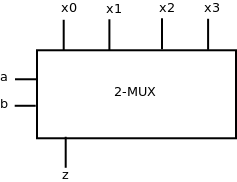
\includegraphics[width=3cm]{3-3.png}
\begin{enumerate}
 \item AND: $x_0=x_1=x_2=0$ and $x_3 = 1$ yields output $z = a \land b$
 \item OR: $x_0 = 0$ and $x_1=x_2=x_3= 1$ yields output $z = a \lor b$
 \item NOT: since NOT is an unary operand $b=0$ and $x_0=1, x_1=0, (x_2=x_3=0)$ yields output $z = \lnot a$
\end{enumerate}


\section{Exercise 4}

\begin{tabular}{|l||l|l|l|l|}\hline
$x_i$ & $y_3$ & $y_2$ & $y_1$ & $y_0$ \\\hline\hline
0 & 0 & 0 & 0 & 0  \\\hline
1 & 0 & 0 & 0 & 1  \\\hline
2 & 0 & 0 & 1 & 0  \\\hline
3 & 0 & 0 & 1 & 1  \\\hline
4 & 0 & 1 & 0 & 0  \\\hline
5 & 0 & 1 & 0 & 1  \\\hline
6 & 0 & 1 & 1 & 0  \\\hline
7 & 0 & 1 & 1 & 1  \\\hline
8 & 1 & 0 & 0 & 0  \\\hline
9 & 1 & 0 & 0 & 1  \\\hline
10 & 1 & 0 & 1 & 0 \\\hline
11 & 1 & 0 & 1 & 1 \\\hline
12 & 1 & 1 & 0 & 0 \\\hline
13 & 1 & 1 & 0 & 1 \\\hline
14 & 1 & 1 & 1 & 0 \\\hline
15 & 1 & 1 & 1 & 1 \\\hline
\end{tabular}
Not solved yet...


\end{document}
